\section*{Arquitectura del Proyecto}

\subsection*{Vista Lógica}
La arquitectura del proyecto se basa en el modelo de tres capas: 
\begin{itemize}
    \item \textbf{Capa de Presentación:} Esta capa es la encargada de mostrar la información al usuario. 
    En esta capa se encuentra la interfaz gráfica con la que interactuara el usuario.
    \begin{center}
        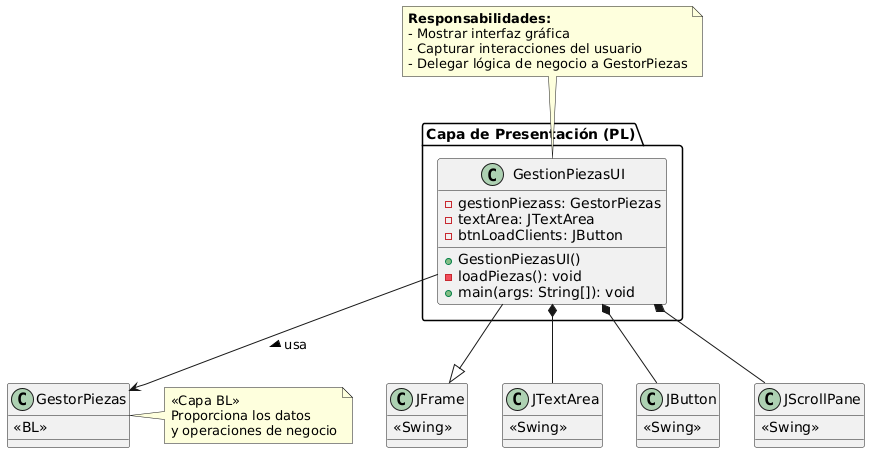
\includegraphics[width=0.8\textwidth]{imag/ImagenDiagramaUmlCapaPresentacion.png}
    \end{center}
    \item \textbf{Capa de Negocio:} Esta capa es la encargada de procesar la información. 
    En esta capa se realizaran todas las funciones del sistema a desarrollar.
    \begin{center}
        
    \end{center}
    \item \textbf{Capa de Acceso a Datos:} Esta capa es la encargada de interactuar con la base de datos. 
    En esta capa se encuentran las consultas a la base de datos.
    \begin{center}
        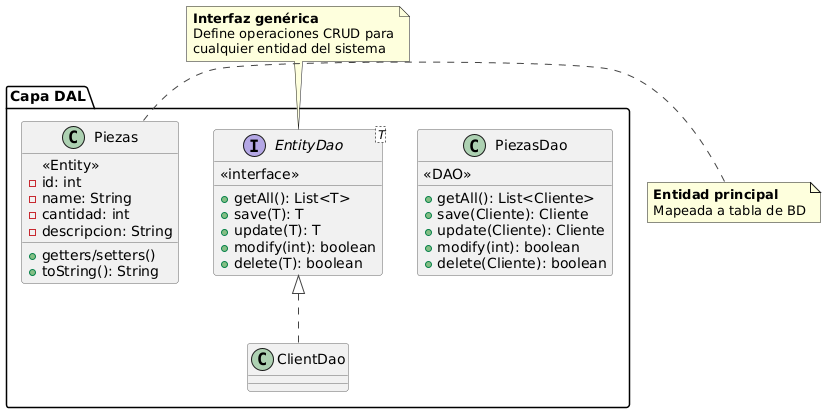
\includegraphics[width=0.8\textwidth]{imag/ImagenDiagramaUmlCapaAccesoDatos.png}
    \end{center}
\end{itemize}

\subsection*{Vista de Casos de Uso}

    La vista de casos de uso se basa en los siguientes casos de uso:
    \begin{itemize}
        \item \textbf{Registrar Refacción:} Este caso de uso permite al usuario registrar una refacción.
        \item \textbf{Modificar Refacción:} Este caso de uso permite al usuario modificar una refacción.
        \item \textbf{Eliminar Refacción:} Este caso de uso permite al usuario eliminar una refacción.
        \item \textbf{Buscar Refacción:} Este caso de uso permite al usuario buscar una refacción.
    \end{itemize}
\subsection*{Planificación UML}
\centering
